\documentclass[../tp2_grupo404.tex]{subfiles}

\graphicspath{{\subfix{../out/}}}

\begin{document}

\subsubsection{Convertir a grafo sin negativos (Bellman-Ford)}
Para el ejemplo tomaremos un grafo G arbitrario. A partir de éste, creamos
un grafo $G^\prime$ idéntico al que le agregamos temporalmente un vértice
$V_0$ con aristas de peso $0$ hacia cada otro nodo preexistente.

\begin{figure}[H]
    \centering
    \subcaptionbox
        {\label{fig:grafoG}\textbf{Grafo $G$ (original)}}
        {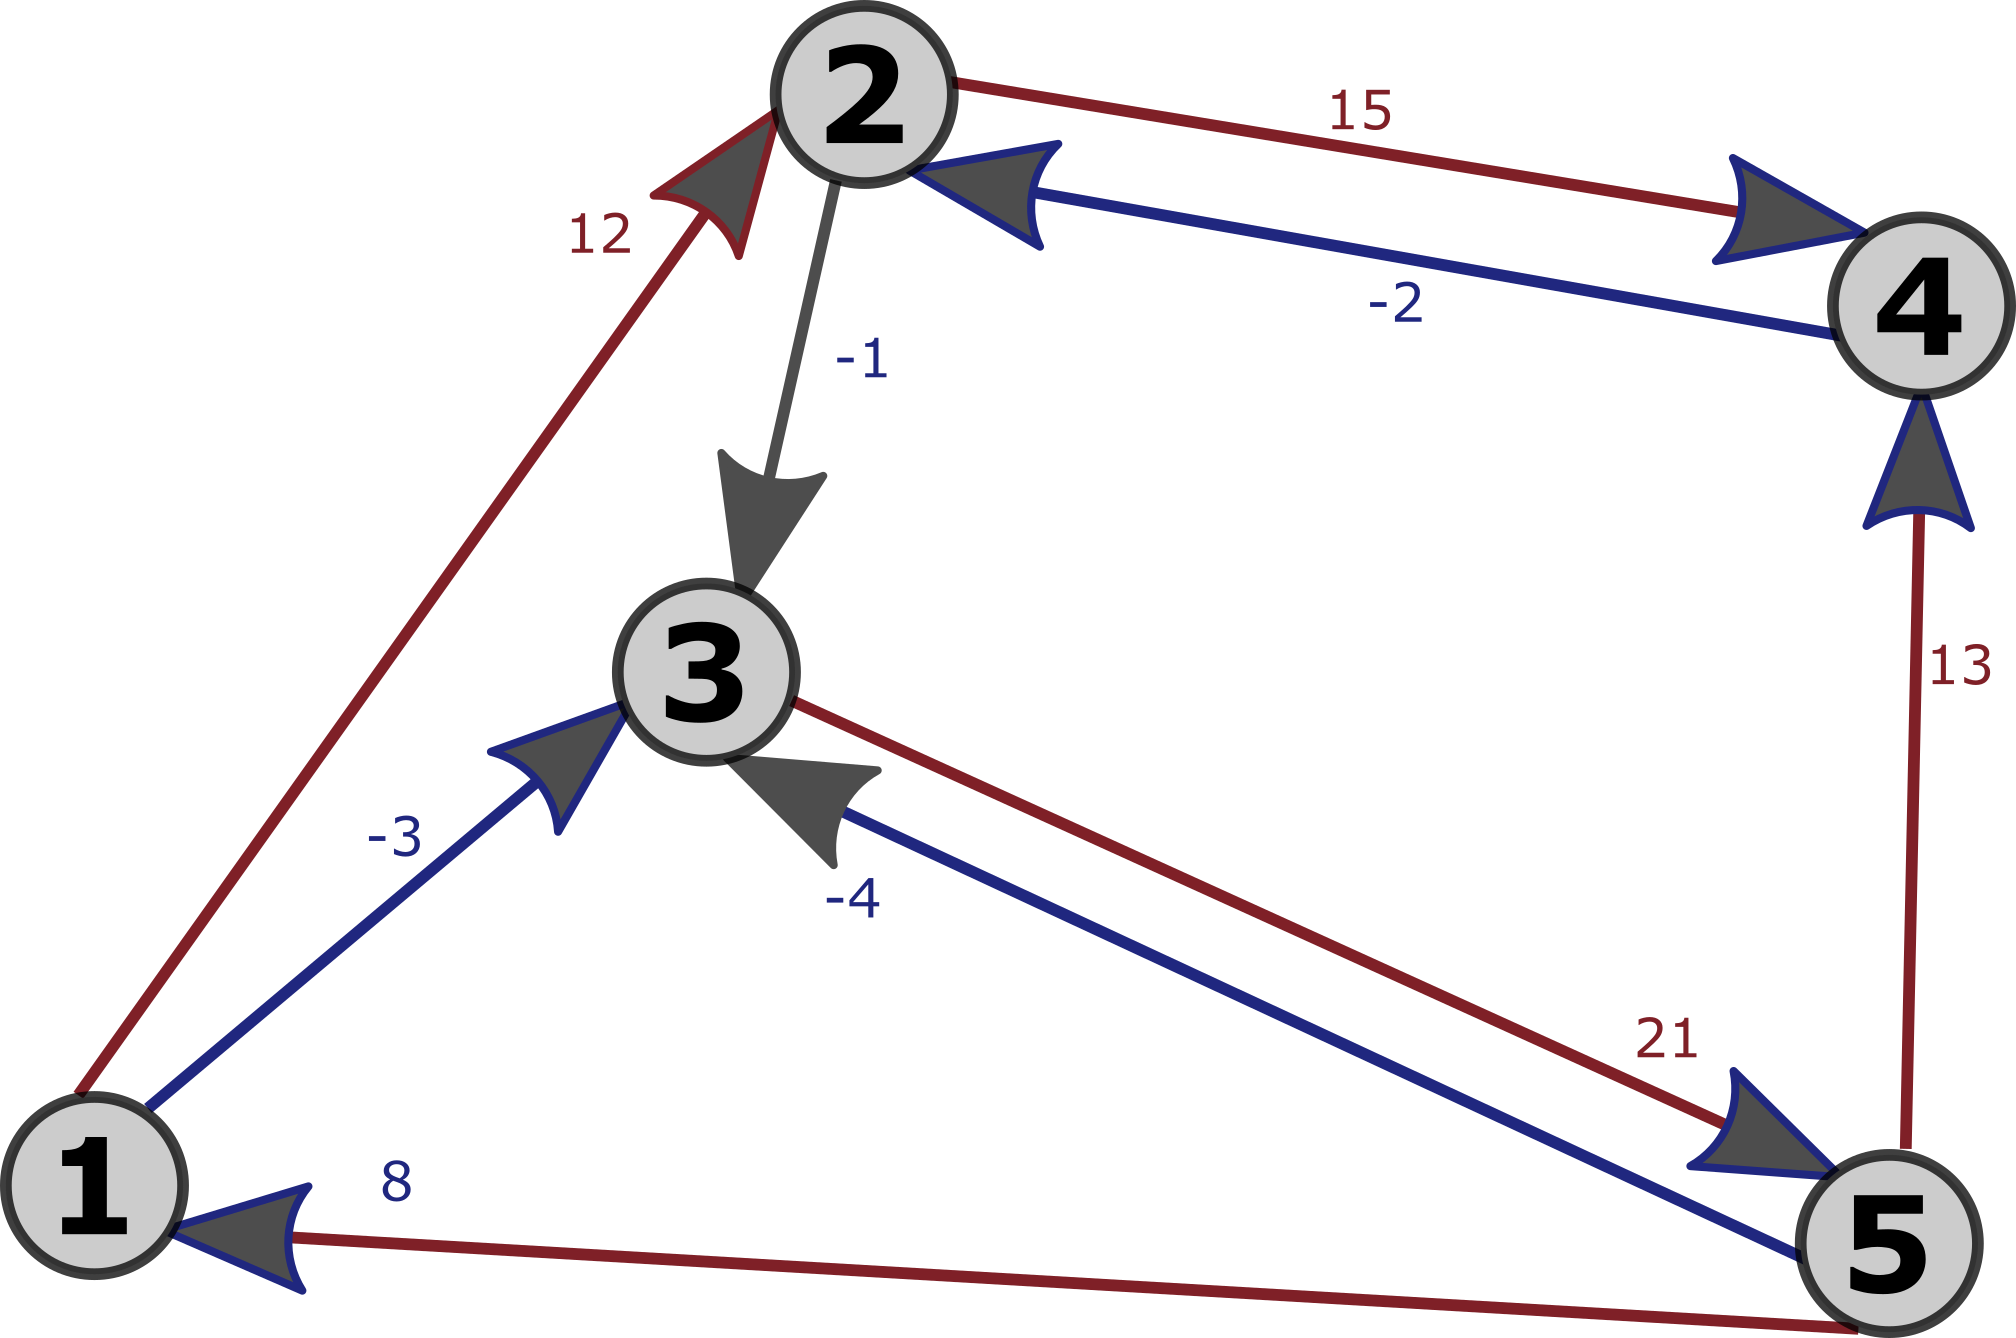
\includegraphics[width=0.4\linewidth,angle=0,origin=c]{out/ford/ford1A.png}}
    \subcaptionbox
        {\label{fig:grafoG_prima}\textbf{Grafo $G^\prime$ (con nodo temporal 0)}}
        {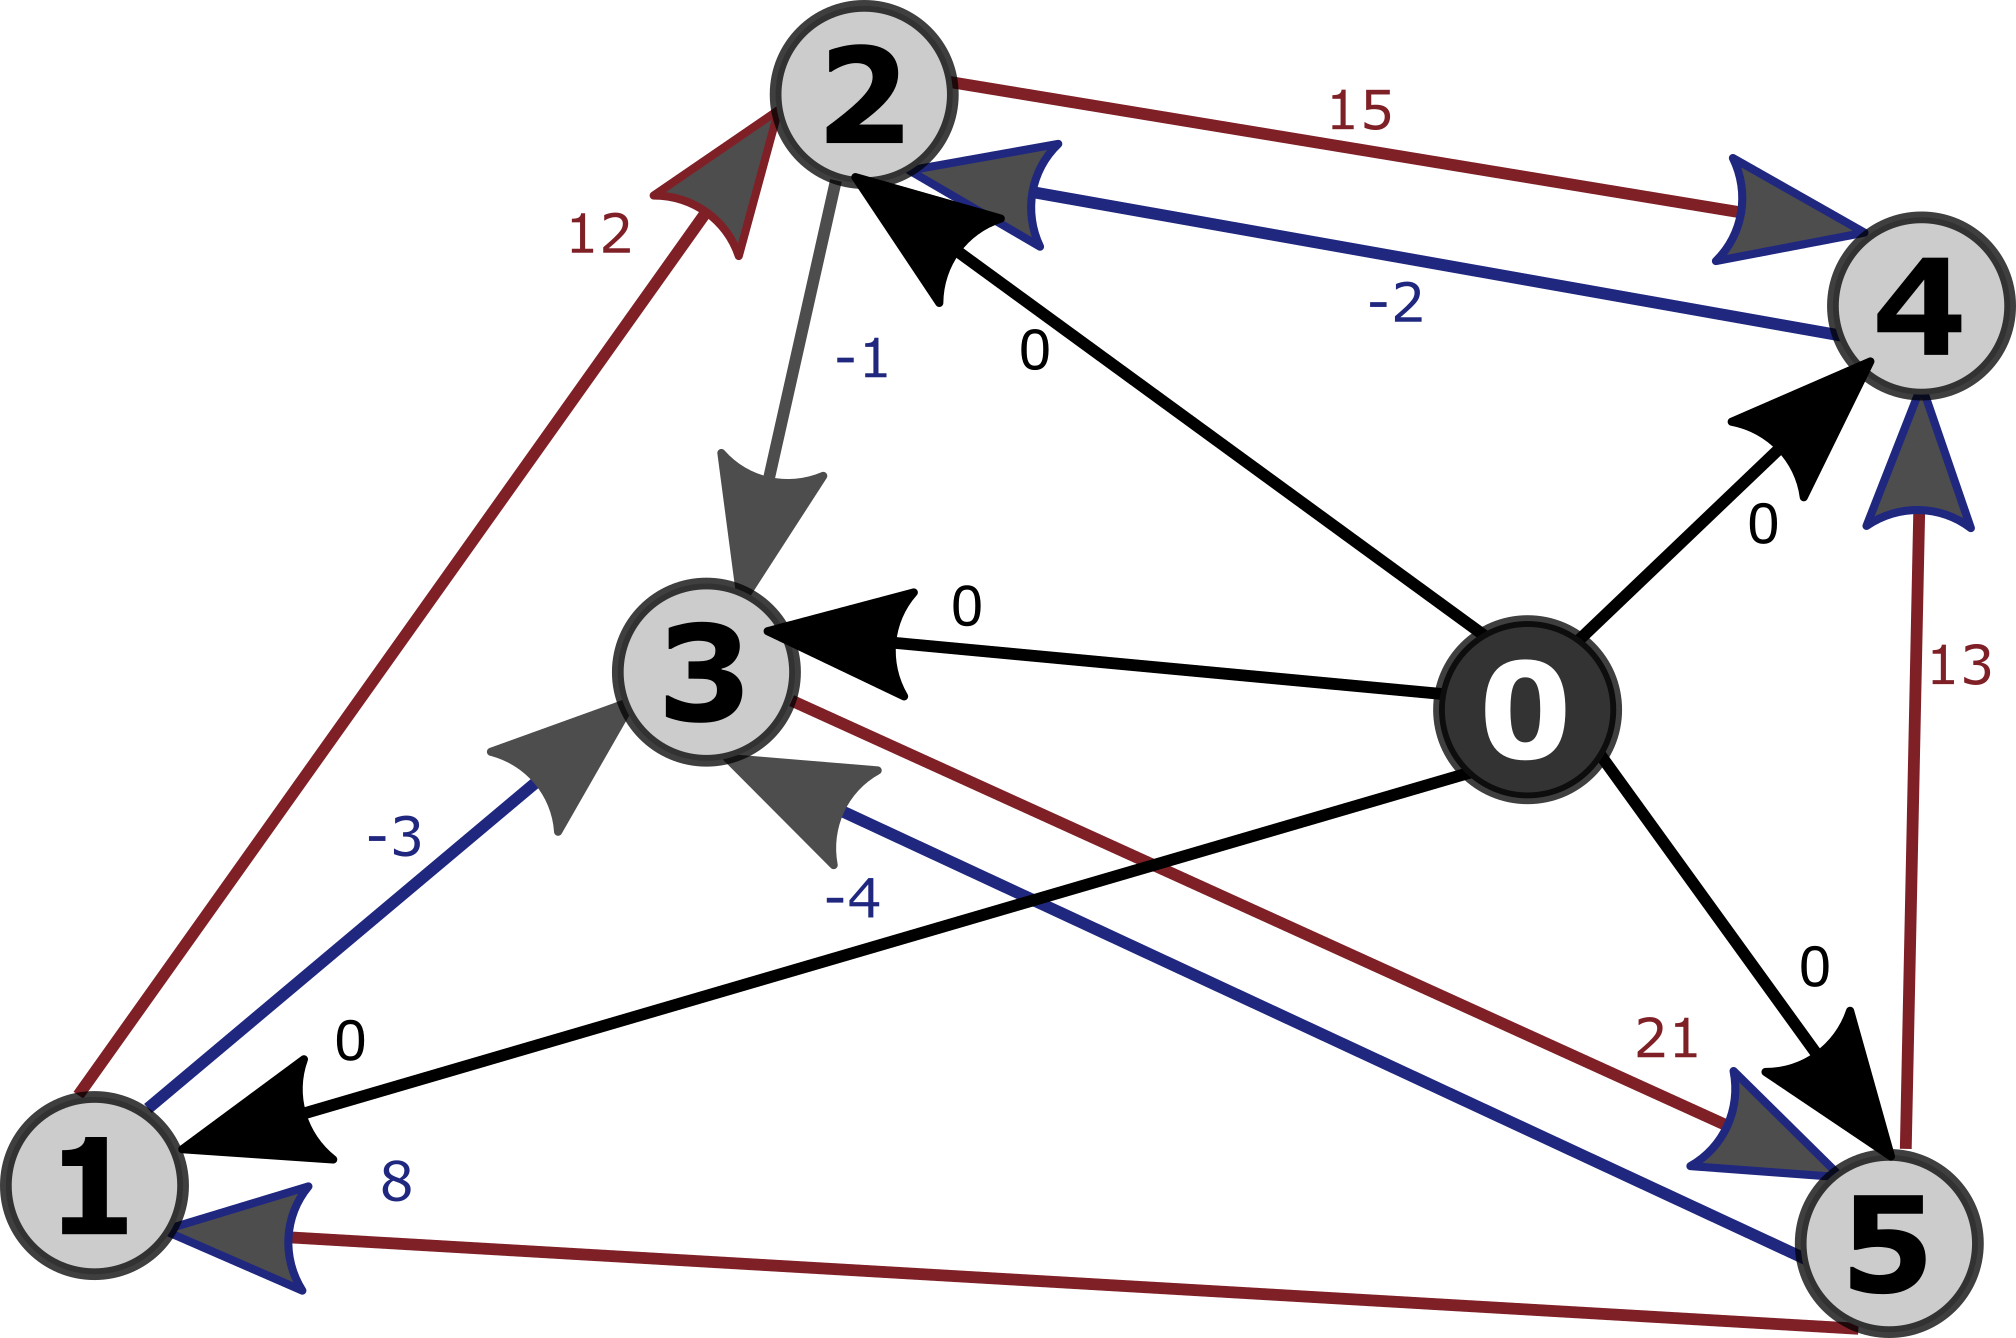
\includegraphics[width=0.4\linewidth,angle=0,origin=c]{out/ford/ford1B.png}}
\end{figure}

A partir de este grafo, aplicamos el algoritmo de Bellman-Ford tomando
como origen el vértice temporal $V_0$. Para el mismo, en cada iteración,
recorreremos todas las aristas haciendo una reducción;
en términos generales:
\begin{displayquote}
Siendo $h(x)$ la distancia al origen estimada para el vértice $x$,
y $w(u,v)$ el peso original de la arista que va desde el vértice $u$ hasta $v$,
comparamos $h(u)+w(u,v)$ contra $h(v$). Si el primer valor es inferior al
segundo, actualizamos $h(v) := h(u)+w(u,v)$ y anotamos $u$ como padre de $v$:
$\pi(v):=u$; esto es, qué otro vértice se tomó para calcular $h(v)$.
\end{displayquote}

Iteramos estas reducciones sobre todas las aristas, un total de
$\lvert V \rvert-1$ veces, y luego una vez más para comprobar que
no haya algún ciclo negativo (que no haya cambios). Adicionalmente,
es posible finalizar con un resultado correcto (es decir, no hay ciclos)
cuando durante una iteración externa no se produjo ningún cambio.
\footnote{Si no hay cambios en la iteración, los datos de entrada de
la siguiente iteración serán los mismos; por lo que el resultado también
será el mismo (y seguirá sin haber cambios). Si bien no modifica
big O, puede reducir el tiempo real de cómputo.}

Como puede observarse en la tabla adjunta, en las primeras
iteraciones simplemente se actualiza la distancia estimada hasta
todos los vértices como cero; esto siempre es así, por definición.
\footnote{Esto es así porque se agregó una arista de peso 0 desde
el origen hasta cada nodo, y las mejores distancias se inicializan
en infinito excepto el origen mismo.}

\begin{table}[H]
    \begin{tabular}{@{}cccccccccccccccccc@{}}
    \toprule
     & \multicolumn{3}{c}{1ª iteración}   & \multicolumn{2}{c}{$V_1$} & \multicolumn{2}{c}{$V_2$}  & \multicolumn{2}{c}{$V_3$} & \multicolumn{2}{c}{$V_4$} & \multicolumn{2}{c}{$V_5$} & \multicolumn{3}{c}{2ª iteración} & \\
     \multirow{-2}{*}{\begin{tabular}[c]{@{}c@{}}Fórmula\\ posible nuevo\end{tabular}}&Nuevo&$\lesseqgtr$& Ant. & h &    p   & h                           & p                             & h                           & p                                    & h & p      & h & p    & Nuevo     & $\lesseqgtr$              & Ant. & \multirow{-2}{*}{Resultados} \\ \cmidrule(r){1-17}
    $0\rightarrow 1 \dots 0\rightarrow 5$   & {\color[HTML]{9A0000} $0+0$} & $<$ & 0                           & 0 & $V_0$ & 0                           & $V_0$                        & 0                           & $V_0$                               & 0 & $V_0$ & 0 & $V_0$ & $0+0$     & $\geq$   & h(x) & Sin cambios                  \\
    $h(1)+w(1,2)$ & $0+12$                          & $<$                     & 0                           & 0 & $V_0$ & 0                           & $V_0$                        & 0                           & $V_0$                               & 0 & $V_0$ & 0 & $V_0$ & $0+12$    & $>$ & $-2$   & Sin cambios                  \\
    $h(1)+w(1,3)$ & {\color[HTML]{9A0000} $0+(-3)$} & {\color[HTML]{9A0000} $<$} & {\color[HTML]{9A0000} $0$}  & 0 & $V_0$ & 0                           & $V_0$                        & {\color[HTML]{9A0000} $-3$} & {\color[HTML]{9A0000} $V_1$} & 0 & $V_0$ & 0 & $V_0$ & $0+(-3)$  & $>$ & $-4$   & Sin cambios                  \\
    $h(2)+w(2,3)$ & $0+-1$                          & $>$                        & -3                          & 0 & $V_0$ & 0                           & $V_0$                        & -3                          & $V_1$                               & 0 & $V_0$ & 0 & $V_0$ & $-2+(-1)$ & $>$ & $-4$   & Sin cambios                  \\
    $h(2)+w(2,4)$ & $0+15$                          & $>$                        & 0                           & 0 & $V_0$ & 0                           & $V_0$                        & -3                          & $V_1$                               & 0 & $V_0$ & 0 & $V_0$ & $-2+15$   & $>$ & $0$    & Sin cambios                  \\
    $h(3)+w(3,5)$ & $-3+21$                         & $>$                        & 0                           & 0 & $V_0$ & 0                           & $V_0$                        & -3                          & $V_1$                               & 0 & $V_0$ & 0 & $V_0$ & $-4+21$   & $>$ & $0$    & Sin cambios                  \\
    $h(4)+w(4,2)$ & {\color[HTML]{9A0000} $0+(-2)$} & {\color[HTML]{9A0000} $<$} & {\color[HTML]{9A0000} $0$}  & 0 & $V_0$ & {\color[HTML]{9A0000} $-2$} & {\color[HTML]{9A0000} $V_4$} & -3                          & $V_1$                               & 0 & $V_0$ & 0 & $V_0$ & $0+(-2)$  & $>$ & $-2$   & Sin cambios                  \\
    $h(5)+w(5,1)$ & $0+8$                           & $>$                        & 0                           & 0 & $V_0$ & -2                          & $V_4$                        & -3                          & $V_1$                               & 0 & $V_0$ & 0 & $V_0$ & $0+8 $    & $>$ & $0$    & Sin cambios                  \\
    $h(5)+w(5,3)$ & {\color[HTML]{9A0000} $0+(-4)$} & {\color[HTML]{9A0000} $<$} & {\color[HTML]{9A0000} $-3$} & 0 & $V_0$ & -2                          & $V_4$                        & {\color[HTML]{9A0000} $-4$} & {\color[HTML]{9A0000} $V_5$} & 0 & $V_0$ & 0 & $V_0$ & $0+(-4)$  & $>$ & $-4$   & Sin cambios                  \\
    $h(5)+w(5,4)$ & $0+13$                          & $>$                        & 0                           & 0 & $V_0$ & -2                          & $V_4$                        & -4                          & $V_5$                               & 0 & $V_0$ & 0 & $V_0$ & $0+13$    & $>$ & $0$    & Sin cambios                  \\ \bottomrule
    \end{tabular}
\end{table}

\begin{table}[H]
    \begin{tabular}{@{}cccccccccccccccccc@{}}
    \toprule
     & \multicolumn{3}{c}{2ª iteración} & \\
     \multirow{-2}{*}{\begin{tabular}[c]{@{}c@{}}Fórmula\\ posible nuevo\end{tabular}}&Nuevo&$\lesseqgtr$& Ant. & \multirow{-2}{*}{Resultados} \\ \cmidrule(r){1-5}
    $0\rightarrow 1 \dots 0\rightarrow 5$   &  $0+0$     & $\geq$   & h(x) & Sin cambios                  \\
    $h(1)+w(1,2)$ & $0+12$    & $>$ & $-2$   & Sin cambios                  \\
    $h(1)+w(1,3)$ & $0+(-3)$  & $>$ & $-4$   & Sin cambios                  \\
    $h(2)+w(2,3)$ & $-2+(-1)$ & $>$ & $-4$   & Sin cambios                  \\
    $h(2)+w(2,4)$ & $-2+15$   & $>$ & $0$    & Sin cambios                  \\
    $h(3)+w(3,5)$ & $-4+21$   & $>$ & $0$    & Sin cambios                  \\
    $h(4)+w(4,2)$ & $0+(-2)$  & $>$ & $-2$   & Sin cambios                  \\
    $h(5)+w(5,1)$ & $0+8 $    & $>$ & $0$    & Sin cambios                  \\
    $h(5)+w(5,3)$ & $0+(-4)$  & $>$ & $-4$   & Sin cambios                  \\
    $h(5)+w(5,4)$ & $0+13$    & $>$ & $0$    & Sin cambios                  \\ \bottomrule
    \end{tabular}
\end{table}
\end{document}
